%
% singularities.tex -- XXX
%
% (c) 2019 Prof Dr Andreas Mueller, Hochschule Rapperswil 
%
\section{Development of singularities\label{burgersunstetig}}
\rhead{Singularities}
\begin{figure}
\begin{center}
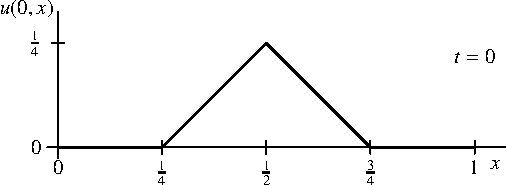
\includegraphics[width=0.8\hsize]{../common/images/burgers-1}
\end{center}
\caption{Anfangsbedingung für die Burgers Gleichung einer idealen
Flüssigkeit\label{burgersanfang}}
\end{figure}
In diesem Abschnitt möchten wir die Burgers Gleichung für die ideale
Flüssigkeit
\[
\frac{\partial}{\partial t}u+\frac{\partial}{\partial x}\left(\frac{u^2}2\right)=0
\]
auf dem Interval $x\in[0,1]$ und für $t>0$
mit der Anfangsbedingung
\[
u(0,x)=\begin{cases}
0\qquad&\text{$x<\frac14$ oder $x>\frac34$}\\
x-\frac14\qquad&\frac14\le x\le \frac12\\
\frac34-x\qquad&\frac12\le x\le \frac34
\end{cases}
\]
lösen (siehe Abbildung \ref{burgersanfang}).

\begin{figure}
\begin{center}
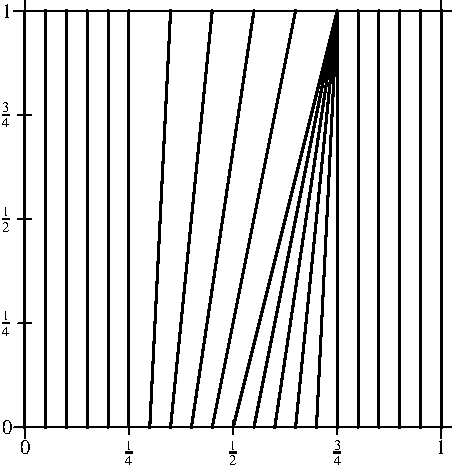
\includegraphics[width=0.8\hsize]{../common/images/burgers-2}
\end{center}
\caption{Niveaulinien (Charakteristiken) der Lösung der Burgers-Gleichung für
die ideale Flüssigkeit\label{burgersniveau}}
\end{figure}
Die Differentialgleichung ist von erster Ordnung, in der Form
\[
\partial_tu+u\partial_xu=0
\]
haben wir die zugehörige geometrische Theorie in Abschnitt
\ref{pdgl1ordnung} besprochen. Dort wurde darauf hingewiesen,
dass der Vektor 
\[
\begin{pmatrix}
1\\u\\0
\end{pmatrix}
\]
immer an die Fläche $u=u(t,x)$ tangential ist. Die Lösungsfläche
entsteht dadurch, dass die Anfangsbedingung mit Hilfe dieses Vektors
verschoben wird. 
Der Punkt $(0,x,u(0,x))$ entwickelt sich nach dieser Methode zu
Punkten $(t,x+u(0,x)t, u(0,x))$ der Lösungsfläche. Die Kurven
gleichen Funktionswertes bilden also Geraden, deren Steigung im
$x$-$t$-Koordinatensystem $u(0,t)^{-1}$ ist. Die Niveaulinien der
Lösung sehen daher aus wie in der Abbildung \ref{burgersniveau}
dargestellt.
Daraus kann man jetzt auch die Lösungen ablesen. In der Abbildung
\ref{burgerssprung} kann man die Entwicklung der Spitze zu einem
Sprung an der Stelle $x=\frac34$ beobachten.

\begin{figure}
\begin{center}
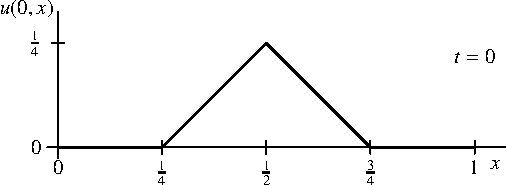
\includegraphics[width=0.8\hsize]{../common/images/burgers-1}
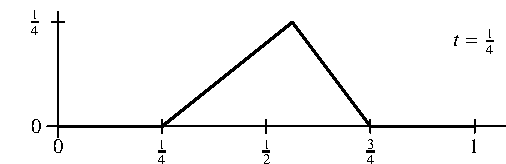
\includegraphics[width=0.8\hsize]{../common/images/burgers-3}
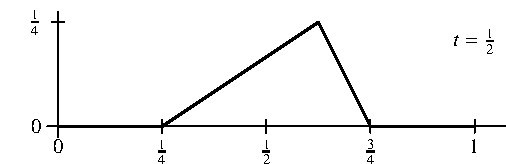
\includegraphics[width=0.8\hsize]{../common/images/burgers-4}
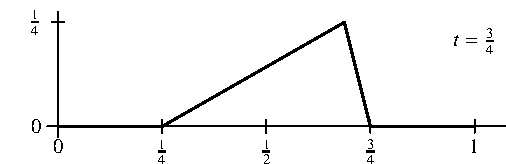
\includegraphics[width=0.8\hsize]{../common/images/burgers-5}
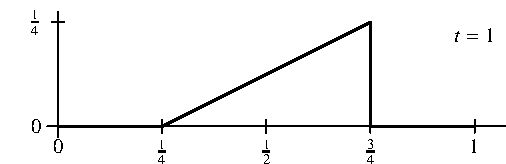
\includegraphics[width=0.8\hsize]{../common/images/burgers-6}
\end{center}
\caption{Entwicklung eines Sprungs in der Lösung der Gleichung von Burgers\label{burgerssprung}}
\end{figure}

Man könnte argumentieren, dass die Anfangsbedingung ja bereits nicht differenzierbar
ist, und dass die Lösungen dies ebenfalls nicht sind. Man kann
jedoch eine beliebige glatte Funktion als Anfangsbedingung wählen, welche
innerhalb des Intervals $[\frac14,\frac12]$ monoton von $0$ auf $\frac14$ 
ansteigt, im Punkt $x=\frac12$ den maximalen Wert $\frac14$ annimmt,
und im Interval $[\frac12,\frac34]$ monoton auf $0$ abfällt.
Das Maximum wird sich entlang der Charakteristiken zum Punkt
$(1,\frac34,\frac14)$ entwicklen. Der Funktionswert $u(0,x)$ im Punkt $(0,x)$
für $x\in[\frac14,\frac12]$ ist derselbe wie im Punkt $(1,x+u(0,x))$.
Der Funktionsgraph $x\mapsto u(1,x)$ hat also die Parameterdarstellung
\[
[{\textstyle\frac14},{\textstyle\frac12}]\to\mathbb R\colon s\mapsto (s+u(0,s),u(0,s))
\]
Diese ist jedenfalls eine glatte Funktion. Andererseits komprimieren
die Charakteristiken das Interval $[\frac12,\frac34]$ auf
den Punkt $(1,\frac34)$ so dass bei $x=\frac34$ wieder ein Sprung entsteht.

